\documentclass[11pt,a4paper]{article}
\usepackage[T1]{fontenc}
\usepackage[utf8]{inputenc}
\usepackage{lmodern}
\usepackage{microtype}
\usepackage[margin=27mm,headheight=15pt]{geometry}
\usepackage{amsmath,amssymb,amsthm,mathtools}
\usepackage{booktabs,tabularx,array}
\usepackage{graphicx}
\usepackage{enumitem}
\usepackage{fancyhdr}
\usepackage{xcolor}
\usepackage{hyperref}
\usepackage{bookmark}
\hypersetup{colorlinks=true,linkcolor=blue!45!black,citecolor=blue!45!black,
 urlcolor=blue!45!black,pdftitle={Dyadic Scaling Rigidity and Log-Periodic Growth of 3AP-Free Permutations},
 pdfauthor={Research article prepared for Vladimir Reshetnikov}}
\pagestyle{fancy}
\fancyhf{}
\fancyhead[L]{\small Dyadic scaling rigidity}
\fancyhead[R]{\small 3AP-free permutations}
\fancyfoot[C]{\thepage}
\setlength{\parskip}{3pt}
\setlength{\parindent}{1.2em}
\setlength{\emergencystretch}{2em}
\setlist[enumerate]{itemsep=4pt,topsep=5pt}
\numberwithin{equation}{section}
\newtheorem{theorem}{Theorem}[section]
\newtheorem{lemma}[theorem]{Lemma}
\newtheorem{proposition}[theorem]{Proposition}
\newtheorem{corollary}[theorem]{Corollary}
\theoremstyle{definition}
\newtheorem{definition}[theorem]{Definition}
\newtheorem{question}[theorem]{Question}
\theoremstyle{remark}
\newtheorem{remark}[theorem]{Remark}
\newcommand{\N}{\mathbb N}
\newcommand{\R}{\mathbb R}
\newcommand{\Z}{\mathbb Z}
\newcommand{\clust}{\operatorname{Clust}}
\newcommand{\supp}{\operatorname{supp}}
\newcommand{\dd}{\,\mathrm d}
\newcommand{\floor}[1]{\left\lfloor#1\right\rfloor}
\newcommand{\ceil}[1]{\left\lceil#1\right\rceil}
\newcommand{\abs}[1]{\left|#1\right|}
\newcommand{\repo}{\textsc{ProveIt}}
\newcommand{\code}[1]{\texttt{\detokenize{#1}}}
\newcommand{\wtag}{\textup{[write]}}
% [write] breakable monospace for long Lean names and paths
\newcommand{\lean}[1]{\nolinkurl{#1}}

\title{\bfseries Dyadic Scaling Rigidity and\newline
Log-Periodic Growth of\newline 3AP-Free Permutations}
\author{Research article prepared for Vladimir Reshetnikov}
\date{September 28, 2026}

\begin{document}
\maketitle
\thispagestyle{empty}
\begin{abstract}
Let $\theta(n)$ count permutations of $[n]$ having no three-term arithmetic
progression as a subsequence. A single exponential growth constant does not
exist, by a theorem of Boon Suan Ho. We determine a more informative asymptotic
object: a unique continuous function $P$, periodic in the binary logarithm,
with
\[
 \log\theta(n)=nP(\log_2 n)-Q(n),\qquad
 \log 2\le Q(n)\le\log 21.
\]
The construction is an application of established divide-and-conquer theory;
an elementary proof with explicit constants is supplied. The central further
result is an exact scale-rigidity theorem. Published enumerative data certify
that $P$ has fundamental period exactly one. Consequently, the positive real
scales $c$ for which
$\log\theta(\lfloor cn\rfloor)-c\log\theta(n)=o(n)$ are precisely the integral
powers of two. At every other scale, exponential gain and exponential loss
both occur on sets of positive lower natural density.
For the concrete split $3n=2n+n$, integer certificates give a factor
$(49/50)^n$ loss when $n=128\cdot2^t$, and a factor $(21/20)^n$ gain when
$n=172\cdot2^t$. We also describe the entire interval of subsequential growth
rates, all cutoff-dependent empirical limit laws, logarithmic averaging,
and polynomial and geometric sampling. A finite-data enclosure algorithm,
reproducible arithmetic certificates, an independent small-count verification,
and a research program complete the article.
\end{abstract}
\vspace{3pt}
\noindent\textbf{Research status.} Unrefereed mathematical development, not a
Lean-verified result. The general periodic-profile method and the failure of a
single growth constant are credited to prior work. The scale-rigidity and
statistical consequences are derived here; their priority in the entire
literature has not been certified. Numerical certificates use published large
counts, independently recomputed in this package only through $n=32$.

\medskip
\noindent\textbf{Collection note} \wtag. This article is the report
\lean{a003407-dyadic-scaling-rigidity} of \repo's research-report collection,
written from one manuscript (batch~40, manuscript~06; see
Section~\ref{dsr:sec:provenance}). None of its own theorems is formalized.
Two inputs that the manuscript takes from the literature, Sharma's upper
splitting bound and the parity lower recurrence, are already proved in Lean
in \repo; Section~\ref{dsr:sec:formal} names the declarations and says what
they do and do not cover. Placement of this report near a Lean development
gives it no formal status. Text added when the report was written is marked
\wtag.
\newpage
\tableofcontents
\newpage

\section{The question and the contribution}
\label{dsr:sec:intro}

\subsection{What should replace a nonexistent growth constant?}
Many counting problems are organized around an asymptotic expression of the
form $C\rho^n n^\alpha$. For three-term-progression-free permutations, even the
coarsest candidate $\rho=\lim\theta(n)^{1/n}$ fails to exist. Merely recording
this failure leaves several natural structural questions unanswered. Does the
sequence exhibit arbitrary exponential-scale oscillation, or a coherent
phase law? Which changes of scale preserve its growth? Can differently sized
blocks be combined at only subexponential cost? Does averaging eliminate the
oscillation?

This article answers these questions in a unified way. The right object is a
continuous growth profile on the circle $\R/\Z$, sampled at the phase
$\log_2 n$. Its period is not just some divisor of one: a short finite
certificate proves that its fundamental period is exactly one. This numerical
shape information has a qualitative consequence for \emph{every real scale},
not merely the finitely many sizes in the table.

Here is the central classification. In this display, $c>0$ is fixed and the
integer $\lfloor cn\rfloor$ is positive for all sufficiently large $n$:
\begin{equation}
\boxed{\quad
 \log\theta(\lfloor cn\rfloor)-c\log\theta(n)=o(n)
 \quad\Longleftrightarrow\quad c\in\{2^j:j\in\Z\}.
 \quad}
\label{dsr:eq:headline}
\end{equation}
Outside these scales, the left side has positive and negative excursions of
order $n$, each occurring on a set of positive lower natural density. Thus the
obstruction is substantially stronger than failure of a ratio limit.

\subsection{Relationship to existing work}
Davis, Entringer, Graham, and Simmons established the parity-splitting
construction for these permutations \cite{DEGS}. Sharma proved the uniform
upper splitting estimate used below \cite[Theorem 2.8]{Sharma}. Correll and
Randy W.~Ho developed dynamic programming and extended the count table
\cite{CorrellHo}; the OEIS table now supplies values through $200$, with later
terms attributed to Alois P.~Heinz \cite{OEIS}.

Boon Suan Ho proved in 2026 that $\theta(n)^{1/n}$ does not converge, by
separating limits along two dyadic subsequences \cite{Ho}. That theorem is
\emph{not} claimed as a result of this article. Separately, Hwang, Janson, and
Tsai give a general theory of continuous periodic fluctuations for
floor/ceiling divide-and-conquer recurrences \cite[Theorem 2.10]{HJT}. Our
profile construction is the equal-weight, bounded-toll specialization of that
theory. We give the proof because the explicit bounds and interpolation are
needed for the subsequent certificates, not because the underlying analytic
principle is new.

The additional contribution developed here consists of the exact period
certificate, the resulting classification \eqref{dsr:eq:headline}, exponential
obstructions to unequal-size gluing, and the complete sampling and empirical
laws for this particular counting sequence. These statements were not found
in the sources inspected for this article. This is a targeted literature
assessment, not a claim of exhaustive priority verification or of resolution
of a separately named published conjecture.

\subsection{Connection with the repository}
\label{dsr:sec:repo}
The selected topic belongs directly to the Ramsey-theoretic part of
\repo~\cite{ProveIt}. In particular, the repository contains the directories
\begin{quote}\small
\code{Combinatorics/Ramsey/Lean/DavisEntringerGrahamSimmons1977/}\par
\code{Combinatorics/Ramsey/Lean/LeSaulnierVijay2011/}.
\end{quote}
The latter statement catalogue, based on \cite{LV}, uses $M(n)$ for the count denoted here by
$\theta(n)$, records the even and odd parity recurrences, and includes the
exponential bounds from the literature. A proposition-valued declaration in a
statement catalogue is not by itself a proved theorem. We therefore take the
published combinatorial estimates as the mathematical input, rather than
inferring proof status from a declaration name.

The inspected repository revision was
\begin{center}\small\code{74f7f5bdba1aa728b340509701a0fa4e45e8dbf3}.
\end{center}
No repository files were changed, and no full Lean build or axiom audit was
performed. The article extends the research direction, not the repository's
machine-checked theorem inventory.

\begin{remark}[Correction \wtag]
\label{dsr:rem:stale-catalogue}\raggedright
The caution above is sound as method, but its conclusion is stale. At the
inspected revision, and unchanged at the time of writing, the declarations in
question are not bare statements. The two parity recurrences are proved as
\lean{LeanProofs.LeSaulnierVijay2011.M_even_recurrence_holds} and
\lean{M_odd_recurrence_holds}, which are derived from the
Davis--Entringer--Graham--Simmons declarations
\lean{even_count_recurrence_holds} and \lean{odd_count_recurrence_holds}.
Sharma's Theorem~2.8, which this article imports, is proved as
\lean{LeanProofs.Sharma2012.theorem_2_8_holds}. The manuscript read only the
statement catalogues, so it did not see these proofs.
Section~\ref{dsr:sec:formal} gives the exact names, files and scope. The
mathematics below is unaffected: both inputs are true and are now also
machine-checked in \repo. The article's own results remain unformalized.
\end{remark}

\subsection{Dependency and verification boundary}
The one substantial theorem imported without reproducing its complete
combinatorial proof is Sharma's upper recurrence. All subsequent analytic and
structural deductions are proved below. The exact-period and explicit-gluing
certificates also use the published count table. The supplied program verifies
the required integer inequalities, but that does not independently prove the
large counts themselves. An independent subset-state enumeration was executed
for every $0\le n\le32$, and direct permutation enumeration for $0\le n\le8$.
These are separate checks with separate evidential roles.

\wtag\ Sharma's recurrence is imported by this article, but it is not an
unchecked input in \repo: its Lean proof is named in
Section~\ref{dsr:sec:formal}. The published count table beyond $n=20$ has no
counterpart in \repo; the Lean development certifies $\theta(1),\ldots,
\theta(20)$ only, whereas the numerical enclosures of
Section~\ref{dsr:sec:reconstruction} and the certificates of
Sections~\ref{dsr:sec:period}--\ref{dsr:sec:rigidity} use published counts
with $100\le n\le200$.

\subsection{Notation, and the names used in the repository \wtag}
\label{dsr:sec:notation}
No symbol of the manuscript has been renamed. The table records the letters
that carry more than one meaning here, or a different meaning in the Lean
developments of \repo, with the tempting false reading beside the true one.
\begin{center}\small
\begin{tabularx}{\linewidth}{@{}l>{\raggedright\arraybackslash}X>{\raggedright\arraybackslash}X@{}}
\toprule
Symbol & Meaning in this article & Remark; tempting false reading\\
\midrule
$\theta(n)$ & number of 3AP-free permutations of $[n]$ (OEIS A003407) &
 equals Lean's \code{Sharma2012.theta n} and the
 \code{M n} of the Davis--Entringer--Graham--Simmons and LeSaulnier--Vijay
 developments (\lean{Sharma2012.theta_eq_davis_count}) \\
$M(x)$ & cutoff-dependent limit of a Ces\`aro mean, $1\le x\le2$
 (Theorem~\ref{dsr:thm:mean-nonconvergence} only) &
 not the count $M(n)=\theta(n)$ of the Lean developments and of
 \cite{DEGS,LV} \\
$R(x)$ & piecewise-affine interpolation of the toll $r_n$,
 \eqref{dsr:eq:R} & not the certificate ratios $R_\pm$ of
 Theorem~\ref{dsr:thm:explicit-gluing} \\
$C$, $C_f$, $C(S)$ & $\int_1^2\Phi$; $\int_1^2 f\circ\Phi$; the
 subset-state continuation count \eqref{dsr:eq:DP} & three different
 objects \\
$Q$ & bounded correction in \eqref{dsr:eq:profile-real}, values in
 $[\log2,\log21]$ & not the toll $r_n$ (whose interpolation is $R$) \\
$L$, $U$, $D$ & the constants $\log2$, $\log21$, $\log(21/2)$ &
 not $\liminf b_n$ and $\limsup b_n$ (those are $p_\pm$) \\
$\gamma$ & $\log_2(21/2)$ in \eqref{dsr:eq:ratio-bound} & an exponent, not
 a growth rate \\
\bottomrule
\end{tabularx}
\end{center}
Unqualified logarithms are natural, and $\log_2$ is the binary logarithm.

\section{Combinatorial input and the bounded toll}
\label{dsr:sec:input}

\begin{definition}
A permutation $\pi=(\pi_1,\ldots,\pi_n)$ of $[n]=\{1,\ldots,n\}$ is
\emph{3AP-free} if there are no indices $i<j<k$ such that
$\pi_i+\pi_k=2\pi_j$. Let $\theta(n)$ be the number of these permutations, with
$\theta(0)=1$. Both increasing and decreasing arithmetic progressions are
forbidden; a progression need not occupy consecutive positions.
\end{definition}
For example, $\theta(1)=1$, $\theta(2)=2$, $\theta(3)=4$, and $\theta(4)=10$.
The distinction between consecutive positions and arbitrary subsequences is
essential to the count.

\begin{lemma}[Parity splitting]
For every integer $n\ge2$,
\begin{equation}
 \theta(n)\ge 2\theta(\lfloor n/2\rfloor)
                         \theta(\lceil n/2\rceil).
\label{dsr:eq:lower}
\end{equation}
\end{lemma}
\begin{proof}
Choose a 3AP-free ordering of the even numbers and one of the odd numbers in
$[n]$, obtained by affine rescaling of smaller 3AP-free permutations.
Concatenate the two blocks, in either order. The two endpoints of any
integer three-term progression have the same parity. If its endpoints were
in one block and its midpoint in the other, the midpoint could not lie
between the endpoints in the concatenated order. If all three entries were
in one block, that block's avoidance property would be violated. Thus both
concatenations avoid three-term progressions. Their orders and their
restrictions to the two nonempty parity blocks determine the input pair, so
the construction counts exactly twice the number of input pairs.
\end{proof}

\begin{theorem}[Sharma's upper splitting bound]
For $n\ge3$,
\begin{equation}
 \theta(n)\le 21\theta(\lfloor n/2\rfloor)
                          \theta(\lceil n/2\rceil).
\label{dsr:eq:upper}
\end{equation}
The same inequality is valid at $n=2$ by direct evaluation.
\end{theorem}
This is \cite[Theorem 2.8]{Sharma}. The proof uses structural restrictions on
how fixed odd and even traces can interleave. We do not replace that
combinatorial theorem by a numerical fit or an unverified recurrence.

\begin{remark}[Formal status of the two inputs \wtag]
\label{dsr:rem:inputs-formal}
Inequality~\eqref{dsr:eq:upper} for $n\ge3$ is the Lean theorem
\lean{LeanProofs.Sharma2012.theorem_2_8_holds}; the case $n=2$ is the direct
evaluation $\theta(2)=2\le21$, which the Lean statement does not include.
Inequality~\eqref{dsr:eq:lower} for all $n\ge2$ is the pair of Lean theorems
\lean{even_count_recurrence_holds} ($n=2k$) and
\lean{odd_count_recurrence_holds} ($n=2k+1$) in the namespace
\lean{LeanProofs.DavisEntringerGrahamSimmons1977}, for $k\ge1$. The proof of
the parity-splitting lemma above is the manuscript's own, and is a second
route to a result already machine-checked. See
Section~\ref{dsr:sec:formal}.
\end{remark}

For the remainder of the paper set
\begin{equation}
 a_n=\log\theta(n),\qquad b_n=\frac{a_n}{n},\qquad
 L=\log2,\quad U=\log21,\quad D=U-L=\log(21/2),
\label{dsr:eq:notation}
\end{equation}
where unqualified logarithms are natural. Define the \emph{toll}
\begin{equation}
 r_n=a_n-a_{\lfloor n/2\rfloor}-a_{\lceil n/2\rceil},\qquad n\ge2.
\label{dsr:eq:toll}
\end{equation}
Equations \eqref{dsr:eq:lower}--\eqref{dsr:eq:upper} say precisely that
\begin{equation}
 L\le r_n\le U. \label{dsr:eq:bounded-toll}
\end{equation}
This is an exact recurrence with a bounded, generally unknown toll; it is not
an assertion that the toll converges or has any simple closed form.

\begin{lemma}[Elementary global bounds]
For every $n\ge1$,
\begin{equation}
 (n-1)L\le a_n\le(n-1)U.
\label{dsr:eq:rough}
\end{equation}
\end{lemma}
\begin{proof}
The assertion holds at $n=1$. If it holds at the two smaller arguments in
\eqref{dsr:eq:toll}, their sizes sum to $n$, and their lower bounds sum to
$(n-2)L$. Adding $r_n\ge L$ gives the lower bound at $n$; the upper bound is
identical with $U$ in place of $L$. Strong induction completes the proof.
\end{proof}

\section{A continuous growth profile with a bounded correction}
\label{dsr:sec:profile}

\subsection{The interpolation identity}
Let $A:[1,\infty)\to\R$ be the piecewise-affine interpolation of $a_n$:
\begin{equation}
 A(n+u)=(1-u)a_n+u a_{n+1},\qquad 0\le u\le1.
\end{equation}
For $x\ge2$, define
\begin{equation}
 R(x)=A(x)-2A(x/2).
\label{dsr:eq:R}
\end{equation}

\begin{lemma}[No interpolation error]
$R$ is the piecewise-affine interpolation of $r_n$. In particular,
\begin{equation}
 L\le R(x)\le U,\qquad
 |R(x)-R(y)|\le\min\{D|x-y|,D\}\quad(x,y\ge2).
\label{dsr:eq:Rbounds}
\end{equation}
\end{lemma}
\begin{proof}
At even integers $n=2m$ we have $2A(n/2)=2a_m$; at odd integers $n=2m+1$ we
have $2A(n/2)=a_m+a_{m+1}$. Thus $R(n)=r_n$ in both cases. On each interval
$[n,n+1]$, both $A(x)$ and $A(x/2)$ are affine: a breakpoint of the latter
can only occur at an even integer. Consequently $R$ is affine there, with
endpoint values $r_n,r_{n+1}$. These values lie in $[L,U]$, so its slope has
absolute value at most $D$, and its entire range has diameter at most $D$.
\end{proof}

\subsection{Construction and uniqueness}
\begin{theorem}[Bounded-error log-periodic law]
\label{dsr:thm:profile}
There is a unique continuous $1$-periodic function $P:\R\to\R$ such that
$a_n=nP(\log_2n)+O(1)$. More precisely, there is a continuous function
$Q:[1,\infty)\to[L,U]$ for which
\begin{equation}
 A(x)=xP(\log_2x)-Q(x),\qquad x\ge1.
\label{dsr:eq:profile-real}
\end{equation}
In particular,
\begin{equation}
 \frac{e^{nP(\log_2n)}}{21}\le\theta(n)
 \le\frac{e^{nP(\log_2n)}}{2},\qquad n\ge1.
\label{dsr:eq:count-envelope}
\end{equation}
Also $L\le P(t)\le U$ for every $t$.
\end{theorem}
\begin{proof}
For $x\ge1$ and $k\ge0$ put $F_k(x)=2^{-k}A(2^kx)$. By
\eqref{dsr:eq:R},
\begin{equation}
 F_{k+1}(x)-F_k(x)=2^{-(k+1)}R(2^{k+1}x).
\end{equation}
The uniform bound on $R$ makes this a uniformly convergent telescoping series,
indeed uniformly on all $x\ge1$. Its limit is
\begin{equation}
 F(x)=A(x)+\sum_{j=1}^{\infty}2^{-j}R(2^jx).
\label{dsr:eq:F}
\end{equation}
Each summand is continuous, so $F$ is continuous. The tail estimate is
\begin{equation}
 L2^{-k}\le F(x)-F_k(x)\le U2^{-k}.
\label{dsr:eq:uniform-tail}
\end{equation}
Shifting the defining limit by one index gives $F(2x)=2F(x)$.

Define $P(t)=2^{-t}F(2^t)$ initially for $t\ge0$. The scaling identity gives
$P(t+1)=P(t)$ and matching endpoint values, so this defines a continuous
$1$-periodic function on all of $\R$. Taking
\begin{equation}
 Q(x)=F(x)-A(x)=\sum_{j\ge1}2^{-j}R(2^jx)
\label{dsr:eq:Q}
\end{equation}
gives $L\le Q(x)\le U$ and proves \eqref{dsr:eq:profile-real}. Exponentiation at
integer $x=n$ gives \eqref{dsr:eq:count-envelope}. Interpolating
\eqref{dsr:eq:rough} and taking the scaled limit gives $Lx\le F(x)\le Ux$,
which proves the asserted bounds on $P$.

For uniqueness, suppose a second continuous $1$-periodic function $P_1$
satisfies the same bounded-error assertion. Fix $t\in[0,1]$ and take
$n_k=\lfloor2^{k+t}\rfloor$. Then $\log_2n_k-k\to t$. Division of both
asymptotic formulas by $n_k$ and continuity imply
$P(t)=\lim b_{n_k}=P_1(t)$. Periodicity extends this equality to every real
argument.
\end{proof}

The theorem is the equal-weight bounded-toll case of the framework in
\cite{HJT}; the proof above makes the constants needed here explicit. The
bound on $Q$ is a genuine uniform multiplicative control on $\theta(n)$,
not just a relative $o(1)$ error in its logarithm. It does \emph{not} assert
that $Q(n)$ converges, so it should not be rewritten as an asymptotic
equivalence with a fixed prefactor.

\subsection{A quantitative modulus of continuity}
Write
\begin{equation}
 \Phi(s)=\frac{F(s)}s=P(\log_2s),\qquad 1\le s\le2.
\end{equation}
We call $s$ the binary mantissa. The endpoints are identified, since
$\Phi(1)=\Phi(2)$.

\begin{proposition}[Explicit log-Lipschitz control]
\label{dsr:prop:modulus}
For $s,t\in[1,2]$, $0<h=|s-t|\le1/2$, and
$J=\lceil\log_2(1/h)\rceil$,
\begin{equation}
 |\Phi(s)-\Phi(t)|
 \le h\bigl[L+U+D(J+1)\bigr].
\label{dsr:eq:modulus}
\end{equation}
Consequently $P$ is H\"older continuous of every exponent less than one, and
has a circle modulus $O(h\log(1/h))$ as $h\downarrow0$.
\end{proposition}
\begin{proof}
On $[1,2]$, $A(s)=L(s-1)$. In the series \eqref{dsr:eq:F}, each of the first $J$
terms changes by at most $Dh$ when $s$ is replaced by $t$, by the Lipschitz
bound in \eqref{dsr:eq:Rbounds}. The remaining terms change by at most
$D\sum_{j>J}2^{-j}=D2^{-J}\le Dh$. Hence
$|F(s)-F(t)|\le Lh+Dh(J+1)$. Finally,
\[
 \left|\frac{F(s)}s-\frac{F(t)}t\right|
 \le |F(s)-F(t)|+Uh,
\]
because $F(t)\le Ut$ and $s,t\ge1$. This proves \eqref{dsr:eq:modulus}.
Composition with $s=2^t$ transfers the estimate to each phase interval.
Across the identified endpoints, split the distance at the endpoint and use
$\Phi(1)=\Phi(2)$. The H\"older assertions follow from
$h\log(1/h)=O_\alpha(h^\alpha)$ for $0<\alpha<1$.
\end{proof}
We do not claim that this modulus is optimal for the particular sequence, or
that $P$ is differentiable, Lipschitz, or nowhere differentiable.

\section{The growth spectrum and finite-data reconstruction}
\label{dsr:sec:reconstruction}

\subsection{Every intermediate growth rate occurs}
Define
\begin{equation}
 p_- =\min_{t\in[0,1]}P(t),\qquad p_+=\max_{t\in[0,1]}P(t),\qquad
 \rho_-=e^{p_-},\quad\rho_+=e^{p_+}.
\end{equation}

\begin{theorem}[Complete subsequential spectrum]
\label{dsr:thm:spectrum}
The sets of subsequential limits are
\begin{equation}
 \clust(b_n)=[p_-,p_+],\qquad
 \clust\bigl(\theta(n)^{1/n}\bigr)=[\rho_-,\rho_+].
\label{dsr:eq:spectrum}
\end{equation}
For each $s\in[1,2]$,
\begin{equation}
 \frac{\log\theta(\lfloor2^ks\rfloor)}{\lfloor2^ks\rfloor}
 \longrightarrow\Phi(s),
\label{dsr:eq:phase-ray}
\end{equation}
with error $O(k2^{-k})$. At an exact integer dyadic ray $n=m2^k$, the error
relative to $P(\log_2m)$ is at most $U/(m2^k)$.
\end{theorem}
\begin{proof}
The identity in Theorem~\ref{dsr:thm:profile} gives
$|b_n-P(\log_2n)|\le U/n$. Every sequence of phases has a convergent
subsequence on the circle, so every cluster value belongs to the range of
$P$. Conversely, $\log_2\lfloor2^ks\rfloor-k\to\log_2s$, proving
\eqref{dsr:eq:phase-ray}. The rounding error in the phase is $O(2^{-k})$;
Proposition~\ref{dsr:prop:modulus} turns it into $O(k2^{-k})$ in the value.
A continuous real function on the circle has a compact interval as its
range. Exponentiation gives the second statement of \eqref{dsr:eq:spectrum}.
On an exact dyadic ray there is no phase rounding, giving the stronger error
bound directly.
\end{proof}
Thus the failure of a single growth constant is organized by a continuum of
phases, rather than by two isolated exceptional subsequences. The exact-period
certificate in the next section will in particular show $p_-<p_+$.

\subsection{A certified enclosure from one dyadic-width band}
\begin{theorem}[Finite-band reconstruction]
\label{dsr:thm:band}
Suppose the counts $\theta(N),\ldots,\theta(2N)$ are known, where $N\ge1$ is an
integer. For every real $x\in[N,2N]$,
\begin{equation}
 \frac{A(x)+L}{x}\le P(\log_2x)\le\frac{A(x)+U}{x}.
\label{dsr:eq:band}
\end{equation}
The two envelopes are separated by at most $D/N$, and the interval of phases
covered has length one. Furthermore,
\begin{align}
 \min_{N\le n\le2N}\frac{a_n+L}{n}
 &\le p_-\le
 \min_{N\le n\le2N}\frac{a_n+U}{n}, \label{dsr:eq:min-band}\\
 \max_{N\le n\le2N}\frac{a_n+L}{n}
 &\le p_+\le
 \max_{N\le n\le2N}\frac{a_n+U}{n}. \label{dsr:eq:max-band}
\end{align}
Each displayed enclosure has width at most $D/N$.
\end{theorem}
\begin{proof}
Equation \eqref{dsr:eq:band} is \eqref{dsr:eq:profile-real} together with
$Q\in[L,U]$. On a unit interval, either envelope has the form
$\alpha+\beta/x$, so its maximum and minimum occur at endpoints (or it is
constant). Thus extrema over the whole band can be taken at integers. Since
$\log_2(2N)-\log_2N=1$, the band traverses every phase, which proves
\eqref{dsr:eq:min-band}--\eqref{dsr:eq:max-band}. Pointwise separation is $D/x\le D/N$;
taking maxima or minima cannot increase this bound.
\end{proof}

The theorem gives a uniform approximation algorithm, not an efficient count
enumeration algorithm. In principle one can compute all needed finite counts
by exhaustive search and hence compute $P$ uniformly, and $p_\pm$ as real
numbers, to any prescribed accuracy. Achieving log-profile error $\varepsilon$
requires counts through $O(\varepsilon^{-1})$ by this bound, but obtaining those
counts may be very expensive.

\begin{figure}[tbp]
\centering
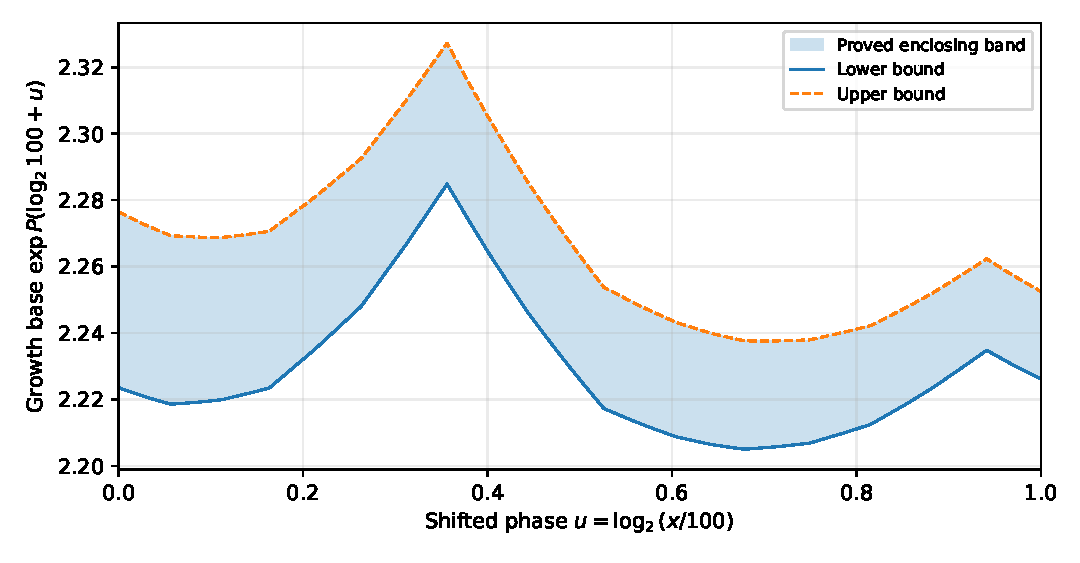
\includegraphics[width=\linewidth]{figures/profile_enclosure.pdf}
\caption{A proved enclosing band from the published counts $100\le n\le200$.
The horizontal coordinate is shifted phase $u=\log_2(x/100)$, not the unshifted
phase $\log_2x$. Both boundaries come from \eqref{dsr:eq:band}; no curve is claimed
to be the exact limiting profile. Plotting uses floating-point arithmetic,
whereas the endpoint and period certificates use exact integers.}
\label{dsr:fig:band}
\end{figure}

\subsection{Numerical bounds with integer verification}
Applying Theorem~\ref{dsr:thm:band} to $100\le n\le200$ gives the following endpoint
expressions. The index selection itself can be checked without logarithms:
compare $B^{1/m}$ and $C^{1/n}$ by comparing $B^n$ and $C^m$.
\begin{center}
\begin{tabular}{@{}lll@{}}
\toprule
Quantity & Certified bounding expression & Decimal approximation\\
\midrule
lower bound for $\rho_-$ & $(2\theta(160))^{1/160}$ & $2.2049986909$\\
upper bound for $\rho_-$ & $(21\theta(162))^{1/162}$ & $2.2375996902$\\
lower bound for $\rho_+$ & $(2\theta(128))^{1/128}$ & $2.2848459606$\\
upper bound for $\rho_+$ & $(21\theta(128))^{1/128}$ & $2.3272067484$\\
\bottomrule
\end{tabular}
\end{center}
In particular, the independently checked rational endpoint inequalities yield
\begin{equation}
 2.20499<\rho_-<2.23760<2.28484<\rho_+<2.32721.
\label{dsr:eq:numeric-bounds}
\end{equation}
These are enclosures, not computed exact values of the extrema. Several of the
same endpoint expressions occur in Ho's analysis \cite{Ho}; numerical
priority is not claimed. The point of the finite-band theorem is that it
certifies the entire profile and gives a systematic error bound, rather than
only selected rays.

\section{A finite certificate for the exact fundamental period}
\label{dsr:sec:period}
The previous sections prove that $P$ is $1$-periodic. A function with period
one could still have period $1/2$, $1/3$, or another smaller period. Excluding
this possibility is essential for the classification of \emph{real} scale
factors in \eqref{dsr:eq:headline}.

\begin{lemma}[Published-data phase gap]
\label{dsr:lem:phase-gap}
The following inequalities hold:
\begin{equation}
 e^{P(0)}>\frac{57}{25}=2.28,
 \qquad
 \sup_{1/4\le t\le1/2}e^{P(t)}<\frac94=2.25.
\label{dsr:eq:phase-gap}
\end{equation}
\end{lemma}
\begin{proof}
All arithmetic needed for the proof is contained in the finite certificate
\begin{align}
 2\theta(128)\,25^{128}&>57^{128}, \label{dsr:eq:gap-cert-one}\\
 21\theta(n)\,4^n&<9^n\qquad(152\le n\le182). \label{dsr:eq:gap-cert-band}
\end{align}
These 32 strict integer inequalities are verified by \code{verify.py} from
the published data \cite{OEIS}. First, $128$ has phase zero, so
Theorem~\ref{dsr:thm:band}, or \eqref{dsr:eq:profile-real} directly, gives
$e^{P(0)}\ge(2\theta(128))^{1/128}>57/25$.

Next, \eqref{dsr:eq:gap-cert-band} says $a_n+U<n\log(9/4)$ at every integer in
$[152,182]$. Linear interpolation therefore gives
$A(x)+U<x\log(9/4)$ throughout that interval. The real interval
\[
 [128\cdot2^{1/4},\,128\sqrt2]
\]
is contained in $[152,182]$: the lower inclusion follows from
$19^4<2\cdot16^4$, and the upper from $2\cdot128^2<182^2$.
For $t\in[1/4,1/2]$, put $x=128\cdot2^t$ and apply the upper envelope.
Periodicity gives $P(\log_2x)=P(7+t)=P(t)$, proving the second inequality.
The bound is uniform and strict because it holds on a compact interval.
\end{proof}

\begin{theorem}[Exact period group]
\label{dsr:thm:period}
The set of periods of $P$ is exactly $\Z$. In particular, its fundamental
positive period is one.
\end{theorem}
\begin{proof}
The phase gap makes $P$ nonconstant. An irrational period $\tau$, together
with period one, would make $P$ constant: the multiples of $\tau$ modulo one
are dense, and continuity propagates the value at any point along that dense
orbit. Thus any additional period must be rational.

If $p/q$ in lowest terms is a period, B\'ezout's identity and period one show
that $1/q$ is a period. Suppose $q\ge2$. There is an integer $j$ with
\begin{equation}
 \frac14\le\frac jq\le\frac12.
\end{equation}
For $q=2,3$ take $j=1$; for $q\ge4$ take $j=\lceil q/4\rceil$.
Period $1/q$ would imply $P(j/q)=P(0)$, contradicting
\eqref{dsr:eq:phase-gap}. Therefore $q=1$. Integer periods already follow from
the construction, completing the proof.
\end{proof}

The certificate proves substantially more than nonconstancy, and it does so
without locating a maximum or minimum. In particular, it does \emph{not}
prove that phase zero is a global maximum. It only proves that a whole
specified phase interval lies below its value, which is enough to rule out
every smaller period at once.

\section{Scaling rigidity and exponential gluing obstructions}
\label{dsr:sec:rigidity}

\subsection{Classification of all positive real scales}
For $c>0$ define, for sufficiently large integers $n$,
\begin{equation}
 T_c(n)=\log\theta(\lfloor cn\rfloor)-c\log\theta(n),
 \qquad
 \Delta_c(t)=P(t+\log_2c)-P(t).
\end{equation}

\begin{lemma}[Uniform phase formula for a scale change]
\label{dsr:lem:scale-formula}
For each fixed $c>0$,
\begin{equation}
 T_c(n)=cn\Delta_c(\log_2n)+O_c(\log n).
\label{dsr:eq:scale-formula}
\end{equation}
If $c$ is an integer, the remainder can be replaced by $O_c(1)$.
\end{lemma}
\begin{proof}
Let $m=\lfloor cn\rfloor$. We have $m=cn+O(1)$ and
$\log_2m=\log_2n+\log_2c+O_c(1/n)$. By
Proposition~\ref{dsr:prop:modulus}, changing the phase by this amount changes $P$
by $O_c(\log n/n)$. Insert this into
$a_m=mP(\log_2m)-Q(m)$, subtract
$ca_n=cnP(\log_2n)-cQ(n)$, and use boundedness of $P$ and $Q$.
If $c$ is integral, there is no rounding and the remainder is exactly
$cQ(n)-Q(cn)$, hence bounded.
\end{proof}

\begin{theorem}[Real-scale rigidity and frequent gain/loss]
\label{dsr:thm:scales}
For $c>0$, $T_c(n)=o(n)$ if and only if $c=2^j$ for an integer $j$.
For every other $c$ there are $\eta_c>0$ and two sets $E_c^+,E_c^-\subseteq\N$
of positive lower natural density such that
\begin{align}
 \theta(\lfloor cn\rfloor)&\ge e^{\eta_cn}\theta(n)^c
                  &&(n\in E_c^+),\label{dsr:eq:scale-plus}\\
 \theta(\lfloor cn\rfloor)&\le e^{-\eta_cn}\theta(n)^c
                  &&(n\in E_c^-).\label{dsr:eq:scale-minus}
\end{align}
Finite initial exceptions may be removed from these sets.
\end{theorem}
\begin{proof}
If $c=2^j$, periodicity makes $\Delta_c$ zero, and
\eqref{dsr:eq:scale-formula} proves $T_c=o(n)$. Conversely, if $T_c=o(n)$, apply
\eqref{dsr:eq:scale-formula} along $n_k=\lfloor2^{k+t}\rfloor$ for each fixed
$t$. Continuity yields $\Delta_c(t)=0$. Thus $\log_2c$ is a period of $P$,
and Theorem~\ref{dsr:thm:period} gives $\log_2c\in\Z$.

Now take an off-dyadic scale. The continuous periodic function $\Delta_c$ is
not identically zero and has integral zero on a period, by translation
invariance of the integral. It therefore has both positive and negative
values. Continuity supplies phase intervals on which $c\Delta_c$ is bounded
below by $2\eta_c$ or above by $-2\eta_c$, for some $\eta_c>0$.
Equation \eqref{dsr:eq:scale-formula} gives \eqref{dsr:eq:scale-plus} and
\eqref{dsr:eq:scale-minus} at all sufficiently large integers with those phases.

For completeness, such phase intervals have positive lower natural density.
Choose a closed mantissa interval $[u,v]\subset(1,2)$ of positive length
inside one of them. If $2^k\le N<2^{k+1}$, the complete dyadic blocks below
$2^k$ contain at least
\[
 (v-u)(2^k-1)-O(k)
\]
integers with mantissa in $[u,v]$. Division by $N<2^{k+1}$ gives lower density
at least $(v-u)/2>0$. Apply this to both sign intervals.
\end{proof}

\begin{corollary}[Integer arities]
\label{dsr:cor:integer-arity}
For an integer $m\ge2$, a uniform subexponential comparison
$\theta(mn)=\theta(n)^m\exp(o(n))$ holds exactly when $m$ is a power of two.
For $m=2^r$ the stronger bounds
\begin{equation}
 2^{m-1}\theta(n)^m\le\theta(mn)\le21^{m-1}\theta(n)^m
\label{dsr:eq:dyadic-amplification}
\end{equation}
hold for every $n\ge1$.
\end{corollary}
\begin{proof}
The classification is Theorem~\ref{dsr:thm:scales}. Iterating the even recurrence
$r$ times gives factors with total exponent $1+2+\cdots+2^{r-1}=m-1$,
which proves \eqref{dsr:eq:dyadic-amplification}.
\end{proof}

There is an important quantifier here: the error $o(n)$ must hold as $n$
runs through \emph{all} sufficiently large integers. Particular off-dyadic
phases can still have zero scale difference. The theorem does not exclude
such accidental equalities of profile values.

\subsection{Explicit exponential failure at the split \texorpdfstring{$2n+n$}{2n+n}}
Define the unequal-block gluing ratio
\begin{equation}
 G(n)=\frac{\theta(3n)}{\theta(2n)\theta(n)}.
\end{equation}
The parity recurrence gives
$\log\theta(2n)-2\log\theta(n)\in[L,U]$, so
\begin{equation}
 \log G(n)=3n\Delta_3(\log_2n)+O(1).
\label{dsr:eq:Gphase}
\end{equation}
In particular, exponential loss and exponential gain for $G(n)$ each occur
on a set of positive lower natural density. The following stronger explicit
subsequences need only four count values.

\begin{theorem}[Certified $2{:}1$ gluing loss and gain]
\label{dsr:thm:explicit-gluing}
For every integer $t\ge0$,
\begin{align}
 G(128\cdot2^t)&<\left(\frac{49}{50}\right)^{128\cdot2^t},
 \label{dsr:eq:explicit-loss}\\
 G(172\cdot2^t)&>\left(\frac{21}{20}\right)^{172\cdot2^t}.
 \label{dsr:eq:explicit-gain}
\end{align}
\end{theorem}
\begin{proof}
Iteration of the even recurrence gives, for $s\ge0$,
\begin{equation}
 2^{2^s-1}\theta(k)^{2^s}\le\theta(k2^s)
 \le21^{2^s-1}\theta(k)^{2^s}.
\label{dsr:eq:iteration}
\end{equation}
Set
\begin{equation}
 R_- =\frac{(21\theta(192))^2}{(2\theta(128))^3},\qquad
 R_+ =\frac{(2\theta(129))^4}{(21\theta(172))^3}.
\end{equation}
The integer certificates checked by the accompanying program are
\begin{align}
 (21\theta(192))^2 50^{128}
  &<(2\theta(128))^3 49^{128},\label{dsr:eq:loss-cert}\\
 (2\theta(129))^4 20^{172}
  &>(21\theta(172))^3 21^{172}.\label{dsr:eq:gain-cert}
\end{align}
Thus $R_-<(49/50)^{128}$ and $R_+>(21/20)^{172}$.

For $n=128\cdot2^t$, write $3n=192\cdot2^{t+1}$. Using the upper bound in
\eqref{dsr:eq:iteration} in the numerator and the lower bounds in the denominator
of $G(n)$ gives
\begin{equation}
 G(n)\le\frac4{21}\,R_-^{2^t}
       <(49/50)^n.
\end{equation}
For $n=172\cdot2^t$, write $3n=129\cdot2^{t+2}$. Use the lower bound for the
numerator and upper bounds for both denominator factors instead. This gives
\begin{equation}
 G(n)\ge\frac{21^2}{2}\,R_+^{2^t}
       >(21/20)^n.
\end{equation}
The prefactors are respectively less than and greater than one, so no
asymptotic threshold is needed: both statements hold for every $t\ge0$.
\end{proof}

\begin{corollary}[No subexponential-loss universal gluing]
There is no function $\varepsilon(N)\to0$ such that, for all sufficiently
large $u,v$,
\begin{equation}
 \theta(u+v)\ge e^{-\varepsilon(u+v)(u+v)}\theta(u)\theta(v).
\end{equation}
Nor does the analogous upper bound with $e^{\varepsilon(u+v)(u+v)}$ hold
uniformly for all large $u,v$.
\end{corollary}
\begin{proof}
Take $u=2n,v=n$ along the loss or gain subsequence in
Theorem~\ref{dsr:thm:explicit-gluing}. The proposed error exponent is $o(n)$,
whereas the exhibited logarithmic discrepancy has magnitude bounded below
by a positive constant times $n$.
\end{proof}

The loss has a direct counting interpretation. Along the first subsequence,
any map from all pairs of 3AP-free permutations of sizes $2n$ and $n$ into
3AP-free permutations of size $3n$ must identify exponentially many pairs
somewhere, if it is defined on the entire domain. In particular, a universal
injective concatenation-type construction at this size ratio is impossible.
This does not rule out successful constructions on a restricted family or
methods that record additional output information.

\section{Averaging and complete empirical limit laws}
\label{dsr:sec:statistics}
The interval of cluster values describes which limits are possible. It does
not describe how often the values occur. Because the phase is logarithmic,
logarithmic and ordinary sampling answer this question differently.

\subsection{Logarithmic averaging has a unique limiting law}
Let $H_N=\sum_{n=1}^N1/n$ and define probability measures
\begin{equation}
 \lambda_N=\frac1{H_N}\sum_{n=1}^N\frac1n\delta_{b_n}.
\end{equation}
Here $\delta_x$ is the point mass at $x$, and convergence of probability
measures means convergence against every continuous test function on a
compact interval containing their supports.

\begin{theorem}[Logarithmic empirical law]
\label{dsr:thm:log-law}
For every continuous test function $f$,
\begin{equation}
 \lim_{N\to\infty}\frac1{H_N}\sum_{n\le N}\frac{f(b_n)}n
   =\int_0^1f(P(t))\dd t
   =\frac1{\log2}\int_1^2 f(\Phi(s))\frac{\dd s}{s}.
\label{dsr:eq:log-law}
\end{equation}
For Lipschitz $f$ the error is $O_f(1/\log N)$. The limiting measure has
support $[p_-,p_+]$. Replacing $b_n$ by $\theta(n)^{1/n}$ pushes this law
forward under the exponential map.
\end{theorem}
\begin{proof}
First take $f$ Lipschitz. Replacing $b_n$ by $P(\log_2n)$ changes the
unnormalized weighted sum by at most
$\operatorname{Lip}(f)U\sum n^{-2}=O_f(1)$.
On $[n,n+1]$, the phase changes by $O(1/n)$, so the modulus of $P$ gives a
change $O(\log n/n)$ in its value. The difference between the resulting sum
and the integral is therefore bounded by a constant times
$\sum_{n\ge2}\log n/n^2$, together with a bounded initial contribution.
Consequently,
\begin{align}
 \sum_{n\le N}\frac{f(b_n)}n
 &=\int_1^N f(P(\log_2x))\frac{\dd x}{x}+O_f(1)\\
 &=(\log N)\int_0^1f(P(t))\dd t+O_f(1),
\end{align}
where the last step splits the logarithmic integral into complete periods
and one bounded remainder. Since $H_N=\log N+O(1)$, this proves the asserted
rate. Continuous test functions follow by uniform approximation by
piecewise-affine, hence Lipschitz, functions on the compact range.

Every neighborhood of a value in the image of a continuous $P$ has a
preimage containing a nonempty phase interval, of positive Lebesgue measure.
Thus the support is the entire image $[p_-,p_+]$. The substitution
$s=2^t$ proves the mantissa formula, and continuity of the exponential gives
the final assertion.
\end{proof}

\subsection{Ordinary cutoffs retain a phase}
Define the ordinary empirical measure
\begin{equation}
 \mu_N=\frac1N\sum_{n=1}^N\delta_{b_n}.
\end{equation}
For $x\in[1,2]$ define a probability measure $\nu_x$ by its test-function
integrals:
\begin{align}
 \nu_x(f)
 &=\frac1x\left(\int_1^2f(\Phi(s))\dd s
                     +\int_1^x f(\Phi(s))\dd s\right)\label{dsr:eq:nu}\\
 &=\frac2x\int_1^x f(\Phi(s))\dd s
      +\frac1x\int_x^2f(\Phi(s))\dd s.\nonumber
\end{align}
The weights integrate to one. At the endpoints $\nu_1=\nu_2$, as required
when the cutoff phase wraps around.

\begin{theorem}[All ordinary empirical limit laws]
\label{dsr:thm:ordinary}
For $N_k=\lfloor2^kx\rfloor$ with $x\in[1,2]$,
\begin{equation}
 \mu_{N_k}\Longrightarrow\nu_x.
\end{equation}
More generally, the complete set of weak subsequential limits of $\mu_N$ is
$\{\nu_x:1\le x\le2\}$. The map $x\mapsto\nu_x$ is weakly continuous and
all its measures have support $[p_-,p_+]$.
\end{theorem}
\begin{proof}
For Lipschitz $f$, replacing $b_n$ by $P(\log_2n)$ changes its ordinary
average by $O_f(H_N/N)$, which tends to zero. Continuous $f$ again follow by
uniform approximation. Put $u_n=n/2^k$. Since $P$ is $1$-periodic,
$P(\log_2n)=P(\log_2u_n)$. Riemann sums on $[\varepsilon,x]$, followed by
$\varepsilon\downarrow0$, give
\begin{equation}
 \lim_{k\to\infty}\mu_{\lfloor2^kx\rfloor}(f)
   =\frac1x\int_0^x f(P(\log_2u))\dd u.
\label{dsr:eq:riemann-law}
\end{equation}
The integrand is bounded and continuous away from zero, so the omitted
interval has arbitrarily small contribution.

Let $C_f=\int_1^2f(\Phi(s))\dd s$. Splitting $(0,1]$ into dyadic intervals
and substituting $u=2^{-j}s$ shows
\begin{equation}
 \int_0^1f(P(\log_2u))\dd u
   =\sum_{j\ge1}2^{-j}C_f=C_f.
\end{equation}
Thus \eqref{dsr:eq:riemann-law} equals \eqref{dsr:eq:nu}.

The same Riemann-sum argument holds for a sequence of upper endpoints
$x_k\to x$, by boundedness of the integrand and the small length of the
interval between $x_k$ and $x$. Every sequence of cutoffs has a subsequence
whose mantissas $N/2^{\lfloor\log_2N\rfloor}$ converge in $[1,2]$.
This proves that no other weak limit is possible, while the fixed-mantissa
cutoffs realize every $\nu_x$. Formula \eqref{dsr:eq:nu} proves weak continuity.
Its mantissa density is at least $1/2$ throughout $[1,2]$, so the support is
the full image of $\Phi$, by the same neighborhood argument used for the
logarithmic law.
\end{proof}

\begin{theorem}[Ordinary averages do not wash out the oscillation]
\label{dsr:thm:mean-nonconvergence}
Neither of the ordinary Ces\`aro averages
\begin{equation}
 \frac1N\sum_{n\le N}\frac{\log\theta(n)}n,
 \qquad
 \frac1N\sum_{n\le N}\theta(n)^{1/n}
\end{equation}
converges. In particular, neither corresponding ordinary empirical measure
has a single weak limit.
\end{theorem}
\begin{proof}
For the first average its cutoff-dependent limit is
\begin{equation}
 M(x)=\frac{C+\int_1^x\Phi(s)\dd s}{x},\qquad
 C=\int_1^2\Phi(s)\dd s.
\end{equation}
Continuity of $\Phi$ makes $M$ continuously differentiable, with
\begin{equation}
 M'(x)=\frac{\Phi(x)-M(x)}x.
\label{dsr:eq:M-ode}
\end{equation}
If $M$ were constant, \eqref{dsr:eq:M-ode} would force $\Phi$ to be constant,
contradicting the phase gap. Thus two cutoff phases give distinct limiting
means. For the second average replace $\Phi$ throughout by $e^\Phi$, which
is likewise continuous and nonconstant. Nonconvergence of these continuous
test-function integrals precludes weak convergence of the empirical measures.
\end{proof}

\begin{remark}
Full support is not the same as existence of a probability density. The
pushforward laws could in principle have atoms at values corresponding to
positive-measure level sets of $P$. Nothing in the arguments above proves
absolute continuity, absence of atoms, or a particular shape of a histogram.
\end{remark}

\section{Polynomial and geometric sampling}
\label{dsr:sec:sampling}

\subsection{Multiplicatively fine sampling preserves the spectrum}
\begin{proposition}
\label{dsr:prop:fine-sampling}
Let $n_k$ be a strictly increasing unbounded sequence of positive integers
with $n_{k+1}/n_k\to1$. Then
\begin{equation}
 \clust(b_{n_k})=[p_-,p_+],\qquad
 \clust\bigl(\theta(n_k)^{1/n_k}\bigr)=[\rho_-,\rho_+].
\end{equation}
In particular this holds along every eventually positive arithmetic
progression with positive common difference and every eventually positive,
nonconstant integer-valued
polynomial sampled at positive integers.
\end{proposition}
\begin{proof}
Fix $s\in[1,2]$ and let $n_{k(j)}$ be the first sample not below $2^js$.
Its predecessor is below $2^js$, so
\[
 1\le\frac{n_{k(j)}}{2^js}
 \le\frac{n_{k(j)}}{n_{k(j)-1}}\longrightarrow1.
\]
Consequently its phases converge to $\log_2s$ modulo one, and the profile
law gives limit $\Phi(s)$. These values fill the interval; no new values are
possible because the sampled sequence is a subsequence of the original.
A polynomial of positive degree and positive leading coefficient is
strictly increasing eventually and has successive ratios tending to one.
Arithmetic progressions are the degree-one case. Removing a finite initial
segment changes none of the assertions.
\end{proof}
This assertion concerns the cluster set, not the frequency distribution
under polynomial sampling. It already shows that the continuum of growth
rates is not confined to specially chosen powers of two.

\subsection{Geometric sampling is governed by rotation}
\begin{theorem}[Geometric sampling classification]
\label{dsr:thm:geometric}
Let $c>0$, $b>1$, $n_k=\lfloor cb^k\rfloor$, and put
$\alpha=\log_2b$, $\beta=\log_2c$. Ignore any initial zero terms.
\begin{enumerate}[label=\textup{(\roman*)}]
\item If $\alpha=p/q$ is rational in lowest terms, the cluster values of
$b_{n_k}$ are
\begin{equation}
 \{P(\beta+jp/q):0\le j<q\},
\end{equation}
and the empirical law is the average of the $q$ corresponding point masses.
Some of the displayed values may coincide.
\item If $\alpha$ is irrational, the cluster set is $[p_-,p_+]$, and
\begin{equation}
 \lim_{K\to\infty}\frac1K\sum_{k=1}^K f(b_{n_k})
       =\int_0^1f(P(t))\dd t
\end{equation}
for every continuous $f$.
\end{enumerate}
Both statements transfer to $\theta(n_k)^{1/n_k}$ by exponentiation.
\end{theorem}
\begin{proof}
Rounding gives
$\log_2n_k=\beta+k\alpha+O(b^{-k})$. The modulus of continuity and bounded
correction imply
\begin{equation}
 b_{n_k}=P(\beta+k\alpha)+O(kb^{-k}).
\end{equation}
In the rational case the phase sequence is periodic with period $q$, and
each residue class of $k$ has frequency $1/q$.

For irrational $\alpha$, each nonzero integer $h$ satisfies
\[
 \frac1K\sum_{k=1}^K e^{2\pi i h(\beta+k\alpha)}\longrightarrow0,
\]
by the finite geometric-sum formula, because
$e^{2\pi i h\alpha}\ne1$. Approximation of continuous periodic functions by
trigonometric polynomials gives uniform distribution of these phases.
Apply it to $f\circ P$. The orbit is dense, so continuity also gives the
full cluster interval. The vanishing rounding error changes neither the
cluster sets nor the limiting averages.
\end{proof}
For example, sampling $n=3^k$ produces the full growth interval and the
logarithmic limiting law, because $\log_2 3$ is irrational. In contrast,
sampling $n=2^k$ converges to the single phase-zero growth value. Exact
fundamental period one does not mean that different phases always have
different values: a continuous real periodic function cannot be injective
on its circle.

\section{Local ratios and the remaining monotonicity problem}
\label{dsr:sec:ratios}
The profile theorem should not be confused with a proof that $\theta(n)$
increases at every step. Ho explicitly distinguishes that open question from
the root-growth question \cite{Ho}. The following exact identity shows where
the difficulty resides.

\begin{proposition}[Binary descent for adjacent logarithmic ratios]
\label{dsr:prop:ratio}
Let $d_n=a_{n+1}-a_n$. Then $d_1=L$, and for $n\ge2$,
\begin{equation}
 d_n=d_{\lfloor n/2\rfloor}+r_{n+1}-r_n.
\label{dsr:eq:d-rec}
\end{equation}
Consequently,
\begin{equation}
 L-D\lfloor\log_2n\rfloor\le d_n
       \le L+D\lfloor\log_2n\rfloor,
\label{dsr:eq:d-bound}
\end{equation}
and, with $\gamma=\log_2(21/2)$,
\begin{equation}
 2n^{-\gamma}\le\frac{\theta(n+1)}{\theta(n)}\le2n^\gamma.
\label{dsr:eq:ratio-bound}
\end{equation}
The elementary deletion bound improves the upper side to $n+1$.
\end{proposition}
\begin{proof}
For $n=2m$, subtract the recurrences for $a_{2m+1}$ and $a_{2m}$; for
$n=2m+1$, subtract those for $a_{2m+2}$ and $a_{2m+1}$. Both subtractions
produce \eqref{dsr:eq:d-rec}. Iteration reaches index one after exactly
$\lfloor\log_2n\rfloor$ steps. Each toll difference is in $[-D,D]$, proving
\eqref{dsr:eq:d-bound}; exponentiation gives \eqref{dsr:eq:ratio-bound}.
For the deletion bound, remove the entry $n+1$ from a 3AP-free permutation
of $[n+1]$. The remaining ordering avoids all progressions in $[n]$. Together
with its original insertion position, this is an injective encoding into
at most $(n+1)\theta(n)$ possibilities.
\end{proof}

The lower bound in \eqref{dsr:eq:ratio-bound} is positive but falls below one; it
therefore does not solve monotonicity. Proving $d_n\ge0$ would require more
information about the correlated toll differences along binary descent than
the independent bounds $r_n\in[L,U]$ supply.

The nondegenerate growth interval also prevents eventual log-convexity or
eventual log-concavity. Either property would make adjacent logarithmic
ratios eventually monotone. The exponential bounds on $a_n$ would then
force their Ces\`aro means $a_n/n$ to converge, contradicting
Theorem~\ref{dsr:thm:spectrum}. This is a limitation of possible regularity
arguments, not a substitute for the unresolved monotonicity question.

\begin{remark}[Adjacent ratios have no limit \wtag]
\label{dsr:rem:ratio}
The same Ces\`aro argument shows that $\theta(n+1)/\theta(n)$ has no limit
in $[0,\infty]$. A finite positive limit $\lambda$ would give
$d_n\to\log\lambda$ and hence $b_n\to\log\lambda$, contradicting
Theorem~\ref{dsr:thm:spectrum} with $p_-<p_+$ (or Ho's theorem \cite{Ho});
the limits $0$ and $\infty$ would force $b_n\to-\infty$ and
$b_n\to+\infty$ respectively, contradicting
\eqref{dsr:eq:rough}. The special case that the ratio does not tend to $2$ is
machine-checked in \repo\ (Section~\ref{dsr:sec:formal}); the general
statement is not formalized. The upper side of
Proposition~\ref{dsr:prop:ratio} is also improved in Lean, to
$\theta(n+1)\le\lfloor(n+3)/2\rfloor\,\theta(n)$.
\end{remark}

\section{Reproducible verification and a formalization route}
\label{dsr:sec:verification}

\subsection{What the package checks}
The program \code{verify.py} uses only the Python standard library. Its
executed record is \code{verification.json}. It performs the following
logically distinct tasks.
\begin{enumerate}
\item It checks all 199 lower and upper splitting inequalities in the supplied
range $2\le n\le200$. These are consistency checks on a finite table, not a
proof of the infinite recurrence.
\item It checks the 32 phase-gap inequalities, the two interval-containment
inequalities, the two explicit gluing certificates, and two previously used
Ho separation certificates, with exact integer arithmetic.
\item It chooses the extremizing indices in each band $[32,64]$, $[64,128]$,
and $[100,200]$ by exact power comparisons. It encloses each selected root
between decimal rationals by integer bisection. Decimal logarithms are used
only to print additional approximations.
\item It independently recomputes $\theta(n)$ for every $0\le n\le32$ using
a subset-state recurrence, and cross-checks $0\le n\le8$ by direct
permutation enumeration.
\end{enumerate}
All these executed checks passed. No claim is made that the independent
Python enumeration was run for $33\le n\le200$, or that a Python assertion is
a proof checked by a theorem prover.

\wtag\ In the collection the program is shipped as \lean{code/verify.py} and
its executed record as \lean{data/verification.json}; the counts are
\lean{data/counts.txt}. The program locates its data relative to its own
directory, so it must be run from a copy that restores the delivered flat
layout (program beside \lean{data/}); the report's README gives the
commands. A rerun of \code{verify.py --max-n 32} on such a copy, made when
the report was written, passed and reproduced the shipped record except for
its timing fields.

\subsection{Why the independent enumeration is correct}
For a fixed $n$, represent the set of values already placed in a prefix by
$S\subseteq[n]$. A candidate next value $y\notin S$ is allowed if, for every
$d\ge1$ with $y-d,y+d\in[n]$, either both endpoints belong to $S$ or neither
does. Equivalently,
\begin{equation}
 \mathbf1_S(y-d)=\mathbf1_S(y+d).
\label{dsr:eq:DP-test}
\end{equation}
Let $C(S)$ be the number of continuations generated by this rule, with
$C([n])=1$ and
\begin{equation}
 C(S)=\sum_{\substack{y\notin S\\y\ \mathrm{allowed}}}C(S\cup\{y\}).
\label{dsr:eq:DP}
\end{equation}
Then $C(\varnothing)=\theta(n)$.

To prove this, consider a complete permutation and a prospective middle
value $y$ of an arithmetic progression. At the moment $y$ is placed, that
progression appears as a subsequence if and only if exactly one of its two
endpoints has already appeared. Thus \eqref{dsr:eq:DP-test} excludes exactly the
forbidden full permutations. Every full permutation corresponds to exactly
one chain of subsets and choices, so \eqref{dsr:eq:DP} counts each permitted
permutation once. The condition depends only on the used set, which justifies
memoization; no unrecorded ordering information is needed for this rule.
This is an independently written implementation of the standard subset-state
idea, not a claim of a new enumeration algorithm \cite{CorrellHo}.

\subsection{Certificate design for a proof assistant}
A practical formalization can be layered rather than beginning with the
analytic limit.

First prove the finite permutation definition, the parity injection, and
soundness of \eqref{dsr:eq:DP}. Next expose Sharma's estimate as an explicit
imported theorem or an explicitly named hypothesis until its full
combinatorial proof has been formalized. Define $a_n$ and $r_n$, prove the
piecewise-affine interpolation lemma, and construct $F$ by uniform convergence
of the geometric tail. This supplies the periodic profile without any
numerical experiments.

The period and gluing proofs then reduce to a small finite certificate over
natural-number powers, plus the already proved interpolation envelope.
A verified certificate evaluator should distinguish ``the table entry is the
count'' from ``the inequality involving that entry is true.'' Finally,
formalize the density and integral arguments on compact intervals. This
separation prevents a conditional analytic theorem from being reported as an
unconditional theorem about the combinatorial sequence.

The present package contains no Lean file asserting these results. The route
just described is an implementation plan, not an executed formalization.

\wtag\ Part of the first layer already exists in \repo, and the second
layer's ``imported theorem'' is not needed there: the permutation
definition, the parity construction and both parity recurrences, the count
identification between the three papers' definitions, and Sharma's
Theorem~2.8 itself are proved in Lean (Section~\ref{dsr:sec:formal}). The
soundness of the subset-state recurrence \eqref{dsr:eq:DP}, the analytic
profile, and every later layer are not formalized. The existing finite-count
evaluator stops at $n=20$ and runs through \lean{native_decide} on a native
backend, which is itself a trust boundary; the certificates above need
$n$ between $100$ and $200$.

\section{Formal status in ProveIt \wtag}
\label{dsr:sec:formal}
This section was added when the report entered the collection. It records
what \repo's Lean development of the three source papers
\cite{DEGS,Sharma,LV} already proves about the objects of this article, and
what it does not. (The Lean namespace \lean{Sharma2012} formalizes the
paper cited here as \cite{Sharma}, 2009.) The Lean files are under
\lean{Combinatorics/Ramsey/Lean/}; the paths below are relative to that
directory, the namespaces begin with \lean{LeanProofs.}, and line numbers
are those of the current tree, which agrees with the manuscript's pinned
revision in this directory. No Lean build and no axiom audit were run for
this report.

\subsection{Declarations that prove inputs of this article}
\begin{itemize}[leftmargin=*,itemsep=3pt]\raggedright
\item \lean{Sharma2012.theorem_2_8_holds}
 (\lean{Sharma2012/FinalConsequences.lean:23}), proving
 \lean{Sharma2012.theorem_2_8} (\lean{Sharma2012/Statements.lean:272}):
 $\theta(n)\le21\,\theta(\lfloor(n+1)/2\rfloor)\,\theta(\lfloor n/2\rfloor)$
 for $n\ge3$. This is \eqref{dsr:eq:upper}, the one theorem the manuscript
 imports. The case $n=2$ is not part of the Lean statement.
\item \lean{DavisEntringerGrahamSimmons1977.even_count_recurrence_holds} and
 \lean{odd_count_recurrence_holds}
 (\lean{DavisEntringerGrahamSimmons1977/CountingRecurrences.lean}, lines 252 and 485):
 $2M(k)^2\le M(2k)$ and $2M(k+1)M(k)\le M(2k+1)$ for $k\ge1$. Together they
 are \eqref{dsr:eq:lower} for every $n\ge2$. The same inequalities are
 restated for Sharma's $\theta$ as \lean{Sharma2012.inequality_1_holds} and
 \lean{inequality_2_holds} (\lean{Sharma2012/CountingConsequences.lean},
 lines 19 and 24) and for LeSaulnier--Vijay's $M$ as
 \lean{LeSaulnierVijay2011.M_even_recurrence_holds} and
 \lean{M_odd_recurrence_holds} (\lean{LeSaulnierVijay2011/Proofs.lean},
 lines 94 and 100).
\item \lean{Sharma2012.theta_eq_davis_count}
 (\lean{Sharma2012/AsymptoticConsequences.lean:22}): Sharma's $\theta$ and the
 Davis--Entringer--Graham--Simmons $M$ are the same count.
\item \lean{Sharma2012.theorem_1_1_holds} and
 \lean{DavisEntringerGrahamSimmons1977.fact_1_holds}:
 $2^{n-1}\le\theta(n)$ for $n\ge1$, the lower half of \eqref{dsr:eq:rough}.
 The upper half, $\theta(n)\le21^{n-1}$, is not stated in Lean; Sharma's
 \lean{theorem_2_9_holds} proves the different bound
 $\theta(n)\le(27/10)^n/21$ for $n\ge11$.
\item \lean{DavisEntringerGrahamSimmons1977.table_1_holds}: the values
 $\theta(1),\ldots,\theta(20)$, which agree with the first twenty entries of
 \lean{data/counts.txt}. They rest on
 \lean{RamseyPaperCommon.reflectedM_values_through_twenty}
 (\lean{RamseyPaperCommon/CountCertificates.lean:17}), proved by
 \lean{native_decide} through an \lean{implemented_by} native backend
 (\lean{RamseyPaperCommon/ThreeFreeCounting.lean}, lines 359--374). These values
 therefore carry that explicit trust boundary. Whether the declarations above
 depend on it was not audited here; the import closure of
 \lean{Sharma2012/FinalConsequences.lean} contains it.
\end{itemize}

\subsection{Declarations bearing on the article's discussion}
\begin{itemize}[leftmargin=*,itemsep=3pt]\raggedright
\item \lean{DavisEntringerGrahamSimmons1977.insertion_count_upper_bound_holds}
 (\lean{DavisEntringerGrahamSimmons1977/Proofs.lean:4824}):
 $\theta(n+1)\le\lfloor(n+3)/2\rfloor\,\theta(n)$ for $n\ge1$. This is
 stronger than the deletion bound $(n+1)\theta(n)$ at the end of
 Proposition~\ref{dsr:prop:ratio}.
\item \lean{LeSaulnierVijay2011.M_ratio_does_not_tend_to_two_holds}
 (\lean{LeSaulnierVijay2011/Proofs.lean:231}): $\theta(n+1)/\theta(n)$ does
 not tend to $2$. This is the negative answer to the question Sharma records
 as \lean{Sharma2012.introduction_ratio_question}. Remark~\ref{dsr:rem:ratio}
 below derives the stronger unformalized statement that the ratio has no
 limit at all.
\item \lean{LeSaulnierVijay2011.theorem_1_holds}:
 $\theta(n)\ge\frac12\,2132^{n/10}$ for $n\ge8$, and Sharma's
 \lean{theorem_2_10_holds}: $\limsup\theta(n)^{1/n}\le27/10$. These are the
 formal exponential bounds. The enclosure \eqref{dsr:eq:numeric-bounds} is
 narrower but rests on published counts that \repo\ does not certify.
\item \lean{Sharma2012.open_problem_1} (monotonicity of $\theta$) and
 \lean{open_problem_2} (convergence of $\theta(n)^{1/n}$)
 (\lean{Sharma2012/Statements.lean}, lines 312 and 316) have no proof declarations, by
 design (\lean{Sharma2012/Proofs.lean}, lines 6--9). The first is still open,
 as Section~\ref{dsr:sec:ratios} says. The second is answered negatively by
 Ho's theorem \cite{Ho}, and again by
 Theorems~\ref{dsr:thm:spectrum} and~\ref{dsr:thm:period}; neither answer is
 formalized, and the Lean docstring correctly describes the question as open
 in Sharma's paper. \lean{open_problem_3}, whether
 $\theta(n+1)<3\theta(n)$ always, is untouched by this article.
\end{itemize}

\subsection{What is not formalized}
None of the article's own results is formalized: the bounded-toll profile
(Theorem~\ref{dsr:thm:profile}), its modulus, the spectrum and band
theorems, the exact period (Theorem~\ref{dsr:thm:period}), the real-scale
classification (Theorem~\ref{dsr:thm:scales}), the explicit gluing
certificates, the empirical and sampling laws, the binary-descent identity,
and the soundness of the subset-state enumeration. The integer certificates
are checked by a Python program only, from published counts that \repo\ does
not certify. Placement of this report beside the Lean development
gives none of these statements formal status.

\section{Further research questions and topics}
\label{dsr:sec:questions}
The results narrow several questions without resolving all of the fine
structure. The following proposed program separates concrete next steps from
more speculative extensions.

\begin{enumerate}[label=\textbf{\arabic*.},leftmargin=*]
\item \textbf{Extremizing phases and sharp constants.}
Determine the exact values or substantially narrower enclosures for
$p_\pm$, and characterize their maximizing and minimizing phase sets. The
certificate used here does not show that $P(0)$ is a global maximum, nor
that either extremum has a unique phase. Larger count bands immediately
produce better certified enclosures, while a structural argument could be
far more informative than additional enumeration.

\item \textbf{Regularity beyond the general bound.}
Is $P$ Lipschitz? Is it differentiable at typical phases, at any dyadic
phase, or on a set of full measure? Is the logarithmic loss in
\eqref{dsr:eq:modulus} actually necessary? These questions require information
about cancellations between toll increments; boundedness alone does not
settle them.

\item \textbf{The distributions of growth values.}
Determine whether the logarithmic pushforward law has atoms, a density, or
a singular component. Study the dependence of the ordinary laws $\nu_x$
on $x$, including when two distinct cutoff phases produce the same law.
The formula \eqref{dsr:eq:nu} is exact, but it does not determine the regularity
of the pushforward without further knowledge of level sets of $P$.

\item \textbf{The bounded multiplicative correction.}
Understand $Q(n)$ and the tolls $r_n$ along dyadic and other arithmetic
subsequences. A limiting correction would strengthen a phase-dependent
exponential envelope to an asymptotic equivalence on that subsequence.
Nothing proved here implies such convergence, and a nontrivial limiting
law for the corrections may be more realistic than a constant prefactor.

\item \textbf{Monotonicity and adjacent ratios.}
Decide whether $\theta(n+1)\ge\theta(n)$ always holds. The binary-descent
identity \eqref{dsr:eq:d-rec} offers a precise target: control a sum of
correlated toll differences, not merely each difference separately.
A combinatorial injection would resolve monotonicity but must accommodate
the unequal-size exponential obstructions proved in this paper.
\wtag\ This is Sharma's open problem~(1), recorded without proof in \repo\
as \lean{Sharma2012.open_problem_1}.

\item \textbf{Sharper interleaving bounds and effective computation.}
Can the uniform factor $21$ be reduced, perhaps beyond a finite threshold,
or replaced by a phase-sensitive bound? Either improvement would sharpen
all the enclosures automatically. Separately, develop an independently
checkable enumeration pipeline for larger count bands with explicit memory,
time, and certificate-size accounting.

\item \textbf{Machine-checked end-to-end certificates.}
Formalize the complete implication from a definition of $\theta$ and a
verified finite-count evaluator to the phase gap, exact period, and gluing
inequalities. The analytic construction is reusable for other balanced
recurrences. The main proof-engineering challenge is avoiding hidden large
count assumptions while keeping the certificate small.
\wtag\ In \repo\ the definition of $\theta$, both splitting recurrences
(including Sharma's upper one) and the values through $n=20$ are already
formalized (Section~\ref{dsr:sec:formal}). What remains is the verified
evaluator for the counts the certificates use ($100\le n\le200$) without a
native trust boundary, the analytic profile, and the certificate
implications themselves.

\item \textbf{Other avoidance classes and generating functions.}
Search for analogous bounded-toll recurrences in longer-progression
avoidance or other permutation classes. Ask whether the resulting profile
can have a smaller fundamental period or whether an exact scale group can
again be read from finite data. For $\sum\theta(n)z^n$, investigate what the
nonconstant exponential profile implies about analytic continuation or
algebraic/differential equations. No non-D-finiteness or natural-boundary
claim is proved here.
\end{enumerate}

\section{Conclusion}
A nonexistent growth constant need not signal unstructured behavior. For
3AP-free permutations, the balanced combinatorial recurrence yields a unique
continuous logarithmic phase profile with a bounded correction. Published
finite data do more than distinguish two limits: they certify the profile's
exact fundamental period. That finite certificate determines the entire
real scaling-symmetry group and forces exponential gain and loss at every
off-dyadic scale.

The explicit $2{:}1$ gluing inequalities show a concrete consequence for
combinatorial constructions, while the empirical laws explain which forms of
averaging preserve or erase the cutoff phase. These results leave the fine
regularity, precise extrema, bounded corrections, and monotonicity of the
counting sequence as well-defined further problems rather than concealing
them inside an unsupported asymptotic ansatz.

\section{Provenance and place in the collection \wtag}
\label{dsr:sec:provenance}
\subsection{Source}
This report was built from \textbf{one} manuscript: manuscript~06 of the
fortieth intake batch of \repo's incoming reports, delivered as the archive
\lean{ProveIt_Dyadic_Scaling_Rigidity.zip} (arrival commit
\lean{017e6c0d8}), dated September 28, 2026, and pinned to \repo\ revision
\lean{74f7f5bdb} (full hash in Section~\ref{dsr:sec:repo} and in the
bibliography). It was placed as a new single-source report in commit
\lean{afb2d1227}. It contributed everything in this article except the text
marked \wtag. No merge was involved, so there were no choices between
sources.

When the report was written, every label received the prefix
\lean{dsr:}; the text marked \wtag\ was added (the collection note, the
correction in Remark~\ref{dsr:rem:stale-catalogue}, the notation table of
Section~\ref{dsr:sec:notation}, Remarks~\ref{dsr:rem:inputs-formal}
and~\ref{dsr:rem:ratio}, Section~\ref{dsr:sec:formal}, short notes in
Sections~\ref{dsr:sec:intro}, \ref{dsr:sec:verification}
and~\ref{dsr:sec:questions} and in the appendix, and this section). No statement, proof, number,
limitation or non-claim of the manuscript was removed or changed, and no
symbol was renamed. The delivered program, data, figure and audit are shipped
byte-identical; their shipped paths are listed in the report's README, and
the delivered audit \lean{SOURCE_AND_PROOF_AUDIT.md} still says that the
Lean catalogue was not checked for proofs, which
Remark~\ref{dsr:rem:stale-catalogue} corrects. The delivered PDF and
checksum ledger are not shipped; this article's PDF is a build of this text.

\subsection{Neighbouring reports}
No other report in \repo's collections treats A003407 or 3AP-free
permutations. Within \lean{oeis-sequence-asymptotics}, the closest contrast is
\lean{a158415-growth-constant}, where a growth constant $\lim a(n)^{1/n}$ is
proved to exist; here none exists, and the periodic profile $P$ takes its
place. The formal neighbour is the Lean development under
\lean{Combinatorics/Ramsey/Lean/} described in
Section~\ref{dsr:sec:formal}.

\appendix
\section{Minimal arithmetic certificate and reproducibility}
The core exact-period certificate can be expressed as the following short
fragment, where \code{theta} is the supplied dictionary of published counts.
No logarithms or floating-point comparisons occur.
\begin{quote}\small
\begin{verbatim}
assert 2 * theta[128] * 25**128 > 57**128
assert 19**4 < 2 * 16**4
assert 2 * 128**2 < 182**2
for n in range(152, 183):
    assert 21 * theta[n] * 4**n < 9**n

assert (21*theta[192])**2 * 50**128 < \
       (2*theta[128])**3 * 49**128
assert (2*theta[129])**4 * 20**172 > \
       (21*theta[172])**3 * 21**172
\end{verbatim}
\end{quote}
The complete program validates the input structure, recomputes small counts,
checks additional consistency and endpoint certificates, and writes a
machine-readable record. To reproduce the executed checks and rebuild the
article, run from the package directory:
\begin{quote}\small
\begin{verbatim}
python verify.py --max-n 32
pdflatex -interaction=nonstopmode -halt-on-error article.tex
pdflatex -interaction=nonstopmode -halt-on-error article.tex
\end{verbatim}
\end{quote}
The existing figure is included in the package. Regeneration with
\code{python plot_profile.py} additionally requires NumPy and Matplotlib;
neither is needed for the exact arithmetic checks. The higher-precision
printed decimals are supplementary to the strict rational enclosures.
\wtag\ These commands assume the delivered flat layout. In the collection the
scripts are in \lean{code/}, so run them on a copy as the report's README
describes; running \lean{code/verify.py} in place fails to find its data.

\begin{thebibliography}{9}
\raggedright
\bibitem{DEGS}
J.~A.~Davis, R.~C.~Entringer, R.~L.~Graham, and G.~J.~Simmons,
\emph{On permutations containing no long arithmetic progressions},
Acta Arithmetica \textbf{34} (1977), 81--90.
\url{https://matwbn.icm.edu.pl/ksiazki/aa/aa34/aa3417.pdf}.

\bibitem{Sharma}
A.~Sharma,
\emph{Enumerating permutations that avoid three term arithmetic progressions},
Electronic Journal of Combinatorics \textbf{16}(1) (2009), \#R63.
\url{https://doi.org/10.37236/152}.
Theorem 2.8 is the upper splitting estimate used here.

\bibitem{LV}
T.~D.~LeSaulnier and S.~Vijay,
\emph{On permutations avoiding arithmetic progressions},
Discrete Mathematics \textbf{311} (2011), 205--207.
\url{https://doi.org/10.1016/j.disc.2010.10.006}.

\bibitem{CorrellHo}
B.~Correll, Jr., and R.~W.~Ho,
\emph{A note on 3-free permutations},
Integers \textbf{17} (2017), A55.
\url{https://arxiv.org/abs/1712.00105}.

\bibitem{Ho}
B.~S.~Ho,
\emph{3AP-free permutations have no exponential growth rate},
arXiv:2602.13617v1 (February 14, 2026).
\url{https://arxiv.org/abs/2602.13617}.

\bibitem{HJT}
H.-K.~Hwang, S.~Janson, and T.-H.~Tsai,
\emph{Identities and periodic oscillations of divide-and-conquer recurrences
splitting at half}, arXiv:2210.10968v1 (2022).
\url{https://arxiv.org/abs/2210.10968}.

\bibitem{OEIS}
The OEIS Foundation Inc., \emph{A003407: Number of permutations of $[n]$
with no 3-term arithmetic progression}.
Table of $n,\theta(n)$ for $0\le n\le200$, attributed to A.~P.~Heinz;
terms through $90$ from B.~Correll, Jr., and R.~W.~Ho.
\url{https://oeis.org/A003407}; data:
\url{https://oeis.org/A003407/b003407.txt}.
Accessed September 28, 2026, Pacific time.

\bibitem{ProveIt}
V.~Reshetnikov, \emph{ProveIt}, GitHub repository.
\url{https://github.com/VladimirReshetnikov/ProveIt}.
Inspected revision
\code{74f7f5bdba1aa728b340509701a0fa4e45e8dbf3};
Ramsey statement catalogues and repository overview. Targeted inspection only;
no full repository build or exhaustive novelty audit.
\end{thebibliography}
\end{document}
